\documentclass[tikz, border = 5pt]{standalone}
\usepackage{tikz}

\usetikzlibrary{arrows.meta}
\usetikzlibrary{shapes.geometric}

\begin{document}

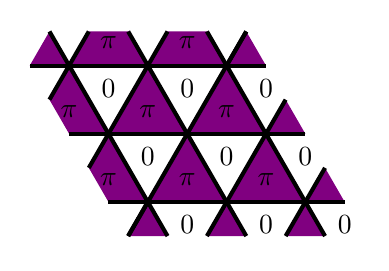
\begin{tikzpicture}[scale = 1.0]

	% model Parameters
	\def \tone{3}	% number of sites in t_1 direction
	\def \ttwo{3} 	% number of sites in t_2 direction
	\def \a{1}	% lattice paramters

	% artistic parameters
	\def \lw{1.5pt}

	% colors
	\definecolor{mypurple}{HTML}{800080}
	\def \uptrcolor{mypurple}

	% get physical coordiantes of points from i and j
	\newcommand{\getpoint}[2]{%
    		\pgfmathsetmacro{\X}{\a*(#1-0.5*#2)}%
    		\pgfmathsetmacro{\Y}{\a*#2*sqrt(3)/2}%
	}
	
	% create lattice points 
	\foreach \i in {1,...,\tone} {
		\foreach \j in {1,...,\ttwo}{
			\getpoint{\i}{\j}
			\coordinate(P-\i-\j) at (\X, \Y);
		}
	}

	% make uptriangles pink 

	\foreach \i in {1,...,\the\numexpr\tone-1\relax}{
		\foreach \j in {1,...,\the\numexpr\ttwo-1\relax}{
			\fill[\uptrcolor] (P-\i-\j) -- (P-\the\numexpr\i+1\relax-\j) -- (P-\the\numexpr\i+1\relax-\the\numexpr\j+1\relax) -- cycle;
		}
	}


	% write pi in uptriangles 
	
	\foreach \i in {1,...,\the\numexpr\tone-1\relax}{
		\foreach \j in {1,...,\the\numexpr\ttwo-1\relax}{
			\getpoint{\i}{\j}
			\pgfmathsetmacro{\Xcord}{\X + 0.5*\a}
			\pgfmathsetmacro{\Ycord}{\Y + \a*0.5/sqrt(3)}
			\node at (\Xcord, \Ycord) {$\pi$};
		}
	}

	% write 0 in downtriangles 

	\foreach \i in {1,...,\the\numexpr\tone-1\relax}{
		\foreach \j in {1,...,\the\numexpr\ttwo-1\relax}{
			\getpoint{\i}{\j}
			\pgfmathsetmacro{\Xcord}{\X}
			\pgfmathsetmacro{\Ycord}{\Y + \a/sqrt(3)}
			\node at (\Xcord, \Ycord) {$0$};
		}
	}

	% make clipped pink trinagles with pi and 0 markings

	% Bottom edge

	\foreach \i in {1,...,\tone}{
		\getpoint{\i}{1}
		\pgfmathsetmacro{\Xright}{\X + 0.25*\a}
		\pgfmathsetmacro{\Xleft}{\X - 0.25*\a}
		\pgfmathsetmacro{\Ybottom}{\Y - sqrt(3)/4*\a}

		\fill[\uptrcolor] (\X, \Y) -- (\Xright, \Ybottom) -- (\Xleft, \Ybottom) -- cycle;

		\pgfmathsetmacro{\Xcord}{\X + 0.5}
		\pgfmathsetmacro{\Ycord}{\Y - 0.5*\a/sqrt(3)}
		\node at (\Xcord, \Ycord) {$0$};
		
	}


	% Top left + Top edge + Top right

	\getpoint{1}{\ttwo}
	\pgfmathsetmacro{\Xleft}{\X-0.5*\a}
	\pgfmathsetmacro{\Xtop}{\X - 0.25*\a}
	\pgfmathsetmacro{\Ytop}{\Y + sqrt(3)/4*\a}

	\fill[\uptrcolor] (\X, \Y) -- (\Xleft, \Y) -- (\Xtop, \Ytop) -- cycle;

	\foreach \i in {1,...,\the\numexpr\tone-1\relax}{
		\getpoint{\i}{\ttwo}
		\pgfmathsetmacro{\Xlefttop}{\X + 0.25*\a}
		\pgfmathsetmacro{\Xrightbottom}{\X+1}
		\pgfmathsetmacro{\Xrighttop}{\X + 0.75*\a}
		\pgfmathsetmacro{\Ytop}{\Y + sqrt(3)/4*\a}

		\fill[\uptrcolor] (\X, \Y) -- (\Xrightbottom, \Y) -- (\Xrighttop, \Ytop) -- (\Xlefttop, \Ytop) -- cycle;

		\pgfmathsetmacro{\Xcord}{\X + 0.5*\a}
		\pgfmathsetmacro{\Ycord}{\Y + \a*0.5/sqrt(3)}
		\node at (\Xcord, \Ycord) {$\pi$};
	}

	\getpoint{\tone}{\ttwo}
	\pgfmathsetmacro{\Xright}{\X+0.5*\a}
	\pgfmathsetmacro{\Xtop}{\X + 0.25*\a}
	\pgfmathsetmacro{\Ytop}{\Y + sqrt(3)/4*\a}

	\fill[\uptrcolor] (\X, \Y) -- (\Xright, \Y) -- (\Xtop, \Ytop) -- cycle;


	% Left edge

	\foreach \j in {1,...,\the\numexpr\ttwo-1\relax}{
		\getpoint{1}{\j}
		\pgfmathsetmacro{\Xbottom}{\X-0.5*\a}
		\pgfmathsetmacro{\Xtop}{\X - 0.75*\a}
		\pgfmathsetmacro{\Ytop}{\Y + sqrt(3)*\a/4}

		\fill[\uptrcolor] (P-1-\j) -- (\Xbottom, \Y) -- (\Xtop, \Ytop) -- (P-1-\the\numexpr\j+1\relax) -- cycle;

		\pgfmathsetmacro{\Xcord}{\X - 0.5*\a}
		\pgfmathsetmacro{\Ycord}{\Y + \a*0.5/sqrt(3)}
		\node at (\Xcord, \Ycord) {$\pi$};
	}

	% Right edge

	\foreach \j in {1,...,\the\numexpr\ttwo-1\relax}{
		\getpoint{\tone}{\j}
		\pgfmathsetmacro{\Xbottom}{\X+0.5*\a}
		\pgfmathsetmacro{\Xtop}{\X + 0.25*\a}
		\pgfmathsetmacro{\Ytop}{\Y + sqrt(3)*\a/4}

		\fill[\uptrcolor] (P-\tone-\j) -- (\Xbottom, \Y) -- (\Xtop, \Ytop) -- cycle;

		\pgfmathsetmacro{\Xcord}{\X}
		\pgfmathsetmacro{\Ycord}{\Y + \a/sqrt(3)}
		\node at (\Xcord, \Ycord) {$0$};
	}


	% Draw nearest neighbour links

	\foreach \i in {1,...,\tone}{
		\foreach \j in {1,...,\ttwo}{
			
			
			\ifnum \i < \tone
				% to right
				\draw[line width = \lw] (P-\i-\j) -- (P-\the\numexpr\i+1\relax-\j);
				\ifnum \j < \ttwo 
					% to top right
					\draw[line width = \lw] (P-\i-\j) -- (P-\the\numexpr\i+1\relax-\the\numexpr\j+1\relax);
				\fi
			\fi


			\ifnum \j < \ttwo
				% to top left
				\draw[line width = \lw] (P-\i-\j) -- (P-\i-\the\numexpr\j+1\relax);
			\fi
		}	
	}

	% Draw half-length nearest neighbour lines outwards from outermost sides

	% Bottom edge
	\foreach \i in {1,...,\tone}{
		\draw[line width = \lw] (P-\i-1) -- ++ (0.25*\a ,{-sqrt(3)/4*\a});
		\draw[line width = \lw] (P-\i-1) -- ++ (-0.25*\a ,{-sqrt(3)/4*\a});
	}
	
	% Top edge
	\foreach \i in {1,...,\tone}{
		\draw[line width = \lw] (P-\i-\ttwo) -- ++ (0.25*\a ,{sqrt(3)/4*\a});
		\draw[line width = \lw] (P-\i-\ttwo) -- ++ (-0.25*\a ,{sqrt(3)/4*\a});
	}

	% Left edge
	\foreach \j in {1,...,\ttwo}{
		\draw[line width = \lw] (P-1-\j) -- ++ (-0.5*\a, 0);
		\draw[line width = \lw] (P-1-\j) -- ++ (-0.25*\a, {-sqrt(3)*\a/4});
	}

	% Right edge
	\foreach \j in {1,...,\ttwo}{
		\draw[line width = \lw] (P-\tone-\j) -- ++ (0.5*\a, 0);
		\draw[line width = \lw] (P-\tone-\j) -- ++ (0.25*\a, {sqrt(3)*\a/4});
	}


	

\end{tikzpicture}

\end{document}

